\begin{tikzpicture}
	% Declare layers
	\pgfdeclarelayer{background}
	\pgfsetlayers{background,main}

	\node (mps) at (0, 0) {\newcommand{\mpsspin}{
	\begin{tikzpicture}
		% filled circle with thick black outline (center fixed at origin)
		\node[draw=black, thick, circle, minimum size=.3cm, inner sep=0pt, fill=\maincolor] (c) at (0,0) {};

	\end{tikzpicture}
}
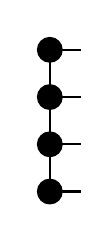
\begin{tikzpicture}
	\def\spindist{.6cm}
	\def\spinout{.4cm}
	% Declare layers
	\pgfdeclarelayer{background}
	\pgfsetlayers{background,main}

	% Spins
	\node (spin1) at (0, 0) {\mpsspin};
	\node (spin2) at ([yshift=-\spindist]spin1) {\mpsspin};
	\node (spin3) at ([yshift=-\spindist]spin2) {\mpsspin};
	\node (spin4) at ([yshift=-\spindist]spin3) {\mpsspin};

	% Line in the background layer
	\begin{pgfonlayer}{background}
		% connection between spins
		\draw[thick] (spin1.center) -- (spin4.center);

		% spin to out
		\draw[thick] (spin1.center) -- ([xshift=\spinout]spin1.center);
		\draw[thick] (spin2.center) -- ([xshift=\spinout]spin2.center);
		\draw[thick] (spin3.center) -- ([xshift=\spinout]spin3.center);
		\draw[thick] (spin4.center) -- ([xshift=\spinout]spin4.center);
	\end{pgfonlayer}
\end{tikzpicture}};
	\node[anchor=west] (cir) at ([xshift=.7cm]mps.east) {\begin{quantikz}[row sep={0.6cm,between origins}, column sep={.9cm,between origins}, background color=\maincolor]
	\ostate & \gate[2]{U^1_1} &                 &                 & [.2cm] \gate[2]{U^2_1} &                 &                 & \ldots \\
	\ostate &                 & \gate[2]{U^1_2} &                 &                        & \gate[2]{U^2_2} &                 & \ldots \\
	\ostate &                 &                 & \gate[2]{U^1_3} &                        &                 & \gate[2]{U^2_3} & \ldots \\
	\ostate &                 &                 &                 &                        &                 &                 & \ldots
\end{quantikz}};
	% background layer
	\begin{pgfonlayer}{background}
		\draw[
		-{Triangle[width=10pt,length=8pt]},
		line width=6pt,
		color=\secondarycolor
		] ([xshift=.2cm]mps.east) -- ([xshift=.1cm]cir.west);
	\end{pgfonlayer}

	\node (d1) at ([yshift=-.15cm, xshift=2.6cm]cir.south west) {$\underbrace{\rule{2.75cm}{0pt}}_{\text{Depth 1}}$};
	\node (d1) at ([yshift=-.15cm, xshift=5.5cm]cir.south west) {$\underbrace{\rule{2.75cm}{0pt}}_{\text{Depth 2}}$};
\end{tikzpicture}